\documentclass[quantumrep,article,accept,oneauthor,pdftex]{Definitions/mdpi} 

%=================================================================
\firstpage{1} 
\makeatletter 
\setcounter{page}{\@firstpage} 
\makeatother
\pubvolume{xx}
\issuenum{1}
\articlenumber{5}
\pubyear{2020}
\copyrightyear{2020}
%\externaleditor{Academic Editor: name}
\history{Published: 12.01.2020}
%\updates{yes} % If there is an update available, un-comment this line

%% MDPI internal command: uncomment if new journal that already uses continuous page numbers 
%\continuouspages{yes}

%------------------------------------------------------------------
% The following line should be uncommented if the LaTeX file is uploaded to arXiv.org
%\pdfoutput=1

%=================================================================
% Add packages and commands here. The following packages are loaded in our class file: fontenc, inputenc, calc, indentfirst, fancyhdr, graphicx,epstopdf, lastpage, ifthen, lineno, float, amsmath, setspace, enumitem, mathpazo, booktabs, titlesec, etoolbox, tabto, xcolor, soul, multirow, microtype, tikz, totcount, amsthm, hyphenat, natbib, hyperref, footmisc, url, geometry, newfloat, caption
\usepackage{subcaption}
\usepackage{braket}

%=================================================================
%% Please use the following mathematics environments: Theorem, Lemma, Corollary, Proposition, Characterization, Property, Problem, Example, ExamplesandDefinitions, Hypothesis, Remark, Definition, Notation, Assumption
%% For proofs, please use the proof environment (the amsthm package is loaded by the MDPI class).

%=================================================================
% Full title of the paper (Capitalized)
\Title{Przygotowanie stanów fotonów o określonej polaryzacji. Transformacja obrotów}

% Authors, for the paper (add full first names)
\Author{Jakub Bąbelek $^{1,\dagger,\ddagger}$}

% Authors, for metadata in PDF
\AuthorNames{Jakub Bąbelek}

% Affiliations / Addresses (Add [1] after \address if there is only one affiliation.)
\address[1]{$^{1}$ \quad Affiliation 1; jakub.babelek@student.out.poznan.pl}

% Abstract (Do not insert blank lines, i.e. \\) 
\abstract{Doświadczenie dotyczy badania superpozycji stanów kwantowych i przygotowania stanu techniką rzutowania oraz badaniu zmiany stanu po obrocie kryształu dwójłomnego. Konsekwencją obrotu kryształu był obrót wiązki rozszczepionej na nadzwyczajną i zwyczajną.}

% Keywords
\keyword{foton; kalcyt; kryształ dwójłomny; transformacja obrotów; fizyka kwantowa; polaryzacja; superpozycja}

%%%%%%%%%%%%%%%%%%%%%%%%%%%%%%%%%%%%%%%%%%
\begin{document}
%%%%%%%%%%%%%%%%%%%%%%%%%%%%%%%%%%%%%%%%%%

%%%%%%%%%%%%%%%%%%%%%%%%%%%%%%%%%%%%%%%%%%
\section{Wstęp}
Doświadczenie wykorzystuje zjawisko dwójłomności, odkryte w 1669 roku przez
Rasmusa Bartholiniego zjawisko dotyczy ono zdolności środków optycznych do
załamywania światła (rozdwojenia promienia świetlnego). Substancje w których
zachodzi te zjawisko nazywamy substancjami dwójłomnymi - są nimi różne formy
substancji krystalicznych w tym niemal wszystkie ciekłe kryształy.

Przykładem substancji dwójłomnych może byc kryształ rutylu lub użyty w poniższym
doświadczeniu kalcyt (Fig.~\ref{fig:kalcyt}).

\begin{figure}[H]
  \centering
  \begin{subfigure}[t]{7cm}
    \centering
    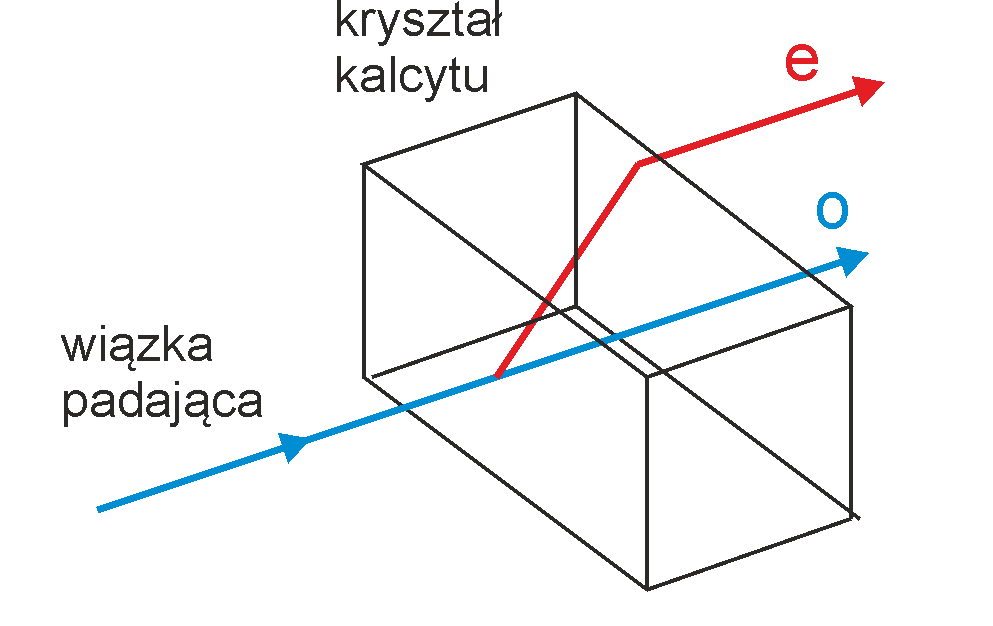
\includegraphics[width=6 cm]{images/dwojlomnosc.png}
  \end{subfigure}%
  ~
  \begin{subfigure}[t]{7cm}
    \centering
    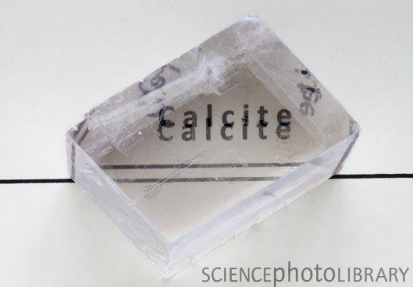
\includegraphics[width=6 cm]{images/kalcyt.png}
  \end{subfigure}
  \caption{\centering Kryształ kalcytu - schemat biegu wiązki i przykład}%
  \label{fig:kalcyt}
\end{figure}

\section{Stanowisko oraz metodyka}
Użyty w doświadczeniu kryształ dwójłomny to kalcyt. Jako źródła światła użyto
lasera, po odbiciu od 2 zwierciadeł wiązka lasera pada na polaryzator a następnie
wspomniany kryształ kalcytu. Wiązka po opuszczeniu kryształu przechodzi przez analizator
i trafia do detektora podłączonego do woltomierza. Cały układ eksperymentalny przedstawiony
został na zdjęciu (Fig.~\ref{fig:stanowisko}).

\begin{figure}[H]
\centering
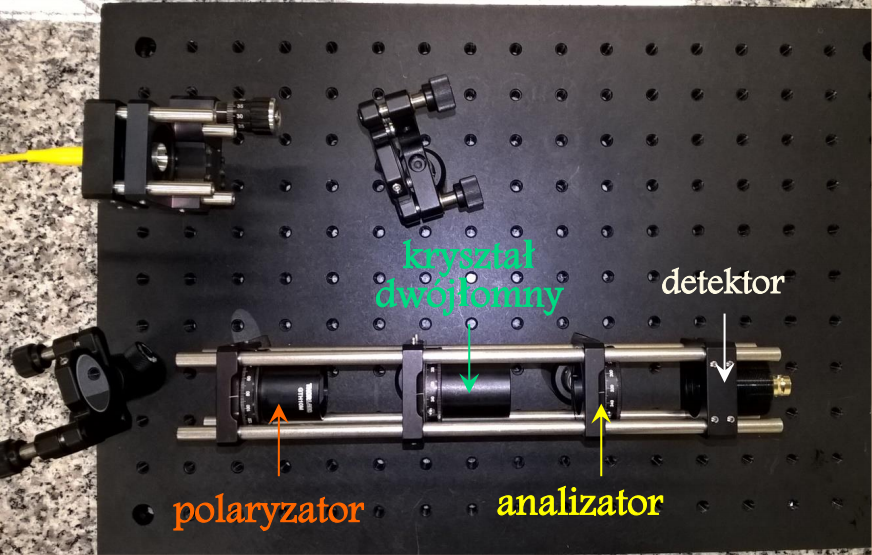
\includegraphics[width=8 cm]{images/stanowisko.png}
\caption{\centering Układ eksperymentalny}%
\label{fig:stanowisko}
\end{figure}

Pomiary przeprowadza się obracając kryształ dwójłomny o określony kąt - \( 10^o \) -
a następnie po poprawnym zidentyfikowaniu wiązek lasera, wygaszenie przy pomocy
analizatora jednej z nich - otrzymując maksimum wiązki widocznej - a następnie
powtórzyć czynność dla drugiej wiązki. Obroty kryształem powodują rotację wiązki
nadzwyczajnej wokół osi symetrii układu.

%%%%%%%%%%%%%%%%%%%%%%%%%%%%%%%%%%%%%%%%%%
\section{Wyniki pomiarów}

\begin{table}[H]
\centering
\begin{tabular}{ccc}
\toprule
\textbf{Kąt obrotu kryształu \( [^o] \)} & \textbf{Napięcie (wiązka nadzwyczajna) \( [mV] \)} & \textbf{Napięcie (wiązka zwyczajna) \( [mV] \)} \\
\midrule
180                                   & 3                                                & 146                                           \\
190                                   & 51                                               & 149                                           \\
200                                   & 87                                               & 144                                           \\
210                                   & 105                                              & 143                                           \\
220                                   & 122                                              & 135                                           \\
230                                   & 132                                              & 124                                           \\
240                                   & 141                                              & 106                                           \\
250                                   & 144                                              & 78                                            \\
260                                   & 146                                              & 35                                            \\
270                                   & 141                                              & 3                                             \\
280                                   & 140                                              & 44                                            \\
290                                   & 135                                              & 84                                            \\
300                                   & 133                                              & 108                                           \\
310                                   & 131                                              & 121                                           \\
320                                   & 120                                              & 134                                           \\
330                                   & 102                                              & 143                                           \\
340                                   & 76                                               & 144                                           \\
350                                   & 33                                               & 145                                           \\
360                                   & 1                                                & 146                                           \\
\bottomrule
\end{tabular}
\caption{Zestawienie wyników pomiarów}%
\label{tab:dane}
\end{table}

Stosując krzywą kalibracyjną dla kryształu dwójłomnego (Fig.~\ref{fig:krzywa})
po podstawieniu wartości napięcia do wzoru (Eq.~\ref{eq:krzywa}), otrzymujemy
wartości mocy wiązki lasera (Fig.~\ref{tab:moc}).

\begin{equation}
  y=y_0 + A_1 e^\frac{x}{t_1}
\label{eq:krzywa}
\end{equation}

\begin{figure}[H]
\centering
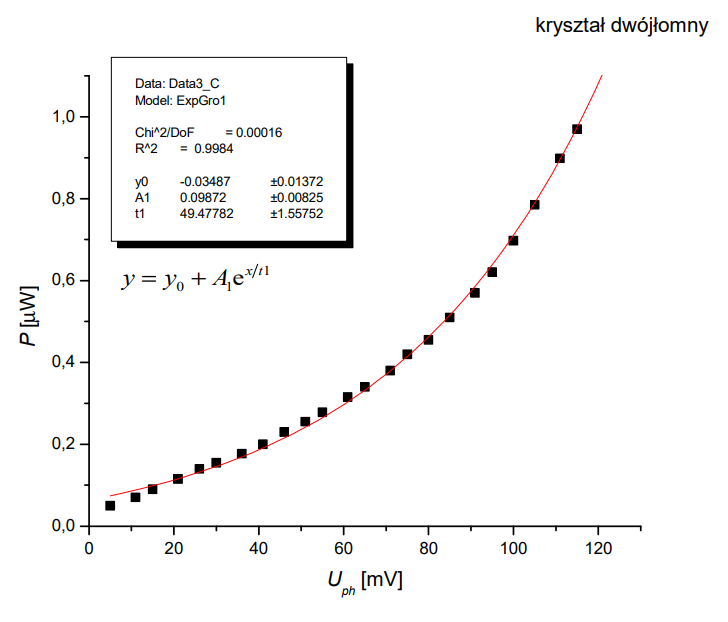
\includegraphics[width=10 cm]{images/krzywa.png}
\caption{\centering Krzywa kalibracji}%
\label{fig:krzywa}
\end{figure}

\begin{table}[H]
\centering
\begin{tabular}{ccccc}
\toprule
\textbf{Kąt obrotu kryształu \( [^o] \)} & \textbf{Moc (nadzwyczajna) \( [\mu W] \)} & \textbf{Moc (zwyczajna) \( [\mu W] \)} \\
\midrule
180                                   & 0.07                                 & 1.85                              \\
190                                   & 0.24                                 & 1.97                              \\
200                                   & 0.54                                 & 1.78                              \\
210                                   & 0.79                                 & 1.74                              \\
220                                   & 1.13                                 & 1.48                              \\
230                                   & 1.39                                 & 1.18                              \\
240                                   & 1.67                                 & 0.81                              \\
250                                   & 1.78                                 & 0.44                              \\
260                                   & 1.85                                 & 0.17                              \\
270                                   & 1.67                                 & 0.07                              \\
280                                   & 1.64                                 & 0.21                              \\
290                                   & 1.48                                 & 0.5                               \\
300                                   & 1.42                                 & 0.84                              \\
310                                   & 1.36                                 & 1.1                               \\
320                                   & 1.08                                 & 1.45                              \\
330                                   & 0.74                                 & 1.74                              \\
340                                   & 0.42                                 & 1.78                              \\
350                                   & 0.16                                 & 1.82                              \\
360                                   & 0.07                                 & 1.85                             \\
\bottomrule
\end{tabular}
\caption{Moc wiązki zwyczajnej oraz nadzwyczajnej}%
\label{tab:moc}
\end{table}

Następnie po użyciu wzoru (Eq.~\ref{eq:norm}) otrzymujemy unormowane wartości mocy (Tab.~\ref{tab:moc_unormowana}).
Równe są prawdopodobieństwu detekcji fotonów dla wzajemnie prostopadłych stanów
polaryzacji.

\begin{equation}
\begin{aligned}
p_e \equiv \left| \alpha_e \right|^2 = \frac{p_e}{p_e + p_o} \\
p_o \equiv \left| \alpha_e \right|^2 = \frac{p_o}{p_o + p_e}
\end{aligned}%
\label{eq:norm}
\end{equation}

\begin{table}[H]
\centering
\begin{tabular}{ccccc}
\toprule
\textbf{Kąt obrotu kryształu \( [^o] \)} & \textbf{Moc unormowana (nadzwyczajna) \( [\mu W] \)} & \textbf{Moc unormowana (zwyczajna) \( [\mu W] \)} \\
\midrule
180                                   & 0.04                                            & 0.96                                         \\
190                                   & 0.11                                            & 0.89                                         \\
200                                   & 0.23                                            & 0.77                                         \\
210                                   & 0.31                                            & 0.69                                         \\
220                                   & 0.43                                            & 0.57                                         \\
230                                   & 0.54                                            & 0.46                                         \\
240                                   & 0.67                                            & 0.33                                         \\
250                                   & 0.8                                             & 0.2                                          \\
260                                   & 0.92                                            & 0.08                                         \\
270                                   & 0.96                                            & 0.04                                         \\
280                                   & 0.89                                            & 0.11                                         \\
290                                   & 0.75                                            & 0.25                                         \\
300                                   & 0.63                                            & 0.37                                         \\
310                                   & 0.55                                            & 0.45                                         \\
320                                   & 0.43                                            & 0.57                                         \\
330                                   & 0.3                                             & 0.7                                          \\
340                                   & 0.19                                            & 0.81                                         \\
350                                   & 0.08                                            & 0.92                                         \\
360                                   & 0.03                                            & 0.97                                         \\
\bottomrule
\end{tabular}
\caption{Unormowana wartość mocy wiązki zwyczajnej oraz nadzwyczajnej}%
\label{tab:moc_unormowana}
\end{table}

Z uzyskanych wartości wykonanujemy wykres zależności \( p_e \) i \( p_o \) od
kąta obrotu kryształu dwójłomnego \( \theta \) (Fig.~\ref{fig:moc_od_kata}) oraz
porównujemy go z wartościami teoretycznymi (Fig.~\ref{fig:cos_sin}) które są
wykresami funkcji \( Sin^2 \theta \) oraz \( Cos^2 \theta \)

\begin{figure}[H]
\centering
\begin{subfigure}[t]{7cm}
\centering
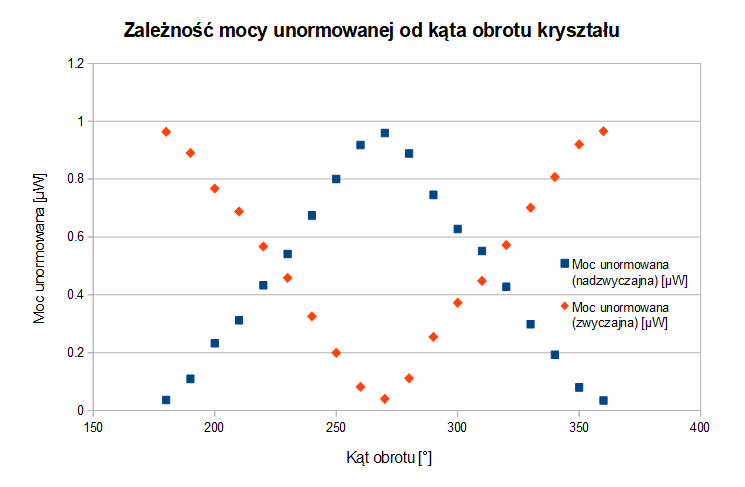
\includegraphics[width=6 cm]{images/moc_od_kata.png}
\caption{\centering Zależność \( p_e \) i \( p_o \) od kąta obrotu kryształu dwójłomnego \( \theta \)}%
\label{fig:moc_od_kata}
\end{subfigure}%
~
\begin{subfigure}[t]{7cm}
\centering
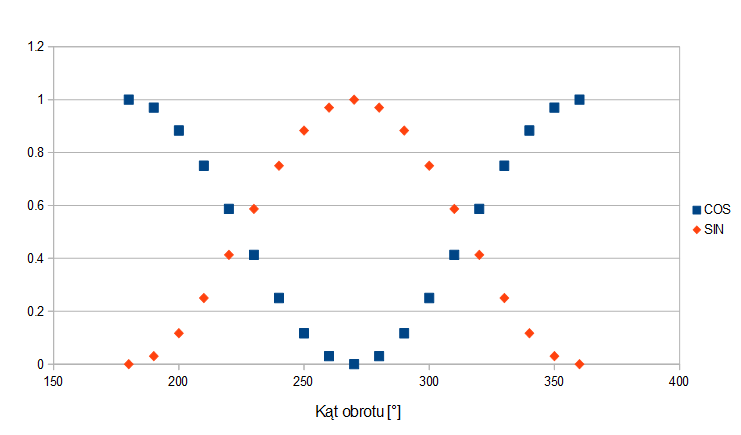
\includegraphics[width=6 cm]{images/cos_sin.png}
\caption{\centering Wykres wartości teoretycznych dla stanu polaryzacji wejściowej \( \ket{V} \)}%
\label{fig:cos_sin}
\end{subfigure}
\caption{\centering Porównanie otrzymanego wykresu z zależnościami teoretycznymi dla stanu polaryzacji wejściowej \( \ket{V} \)}%
\label{fig:zestawienie}
\end{figure}

%%%%%%%%%%%%%%%%%%%%%%%%%%%%%%%%%%%%%%%%%%
\section{Wnioski}
Zestawienie wyników z wartościami oczekiwanymi (Fig.~\ref{fig:zestawienie}) pokazuje
poprawność wykonanego doświadczenia - wykresy doświadczalne i wartości teoretyczne pokrywają
się ze sobą. Pomimo niewiekich różnic spowodowanych zapewne przez niedokładność
układu pomiarowego czy brak odpowiednich warunków (półmrok) uzyskano zamierzony
efekt.

%%%%%%%%%%%%%%%%%%%%%%%%%%%%%%%%%%%%%%%%%%
\vspace{6pt} 

%%%%%%%%%%%%%%%%%%%%%%%%%%%%%%%%%%%%%%%%%%
\funding{This research received no external funding}

%%%%%%%%%%%%%%%%%%%%%%%%%%%%%%%%%%%%%%%%%%
\acknowledgments{Poznan University of Technology - laboratory and equipment used to make the experiment}

%%%%%%%%%%%%%%%%%%%%%%%%%%%%%%%%%%%%%%%%%%
\conflictsofinterest{The authors declare no conflict of interest} 

\newpage
%%%%%%%%%%%%%%%%%%%%%%%%%%%%%%%%%%%%%%%%%%
\reftitle{References}

% Please provide either the correct journal abbreviation (e.g. according to the “List of Title Word Abbreviations” http://www.issn.org/services/online-services/access-to-the-ltwa/) or the full name of the journal.
% Citations and References in Supplementary files are permitted provided that they also appear in the reference list here. 

%=====================================
% References, variant A: external bibliography
%=====================================
%\externalbibliography{yes}
%\bibliography{your_external_BibTeX_file}

%=====================================
% References, variant B: internal bibliography
%=====================================
\begin{thebibliography}{999}
\bibitem{}
Zbigniew Kąkol; Piotr Morawski, Dwójłomność,Open AGH E-Podręczniki 2019
\bibitem{}
M.J. Steel, T.P. White, C. Martijn de Sterke, R.C. McPhedran, L.C. Botten, Symmetry and degeneracy in mictrosructured optical fibers, Opt. Lett. 26 (2001), s. 488–490.
\bibitem{}
Thompson, D. W.; Devries, M. J.; Tiwald, T. E.; Woollam, J. A. (1998). "Determination of optical anisotropy in calcite from ultraviolet to mid-infrared by generalized ellipsometry". Thin Solid Films. 313–314 (1–2): 341–346. 
\end{thebibliography}

% The following MDPI journals use author-date citation: Arts, Econometrics, Economies, Genealogy, Humanities, IJFS, JRFM, Laws, Religions, Risks, Social Sciences. For those journals, please follow the formatting guidelines on http://www.mdpi.com/authors/references
% To cite two works by the same author: \citeauthor{ref-journal-1a} (\citeyear{ref-journal-1a}, \citeyear{ref-journal-1b}). This produces: Whittaker (1967, 1975)
% To cite two works by the same author with specific pages: \citeauthor{ref-journal-3a} (\citeyear{ref-journal-3a}, p. 328; \citeyear{ref-journal-3b}, p.475). This produces: Wong (1999, p. 328; 2000, p. 475)


%%%%%%%%%%%%%%%%%%%%%%%%%%%%%%%%%%%%%%%%%%

%% for journal Sci
%\reviewreports{\\
%Reviewer 1 comments and authors’ response\\
%Reviewer 2 comments and authors’ response\\
%Reviewer 3 comments and authors’ response
%}

%%%%%%%%%%%%%%%%%%%%%%%%%%%%%%%%%%%%%%%%%%
\end{document}

